\section{Results}
\label{sec:results}

This section consolidates the headline quantitative results from all four
milestones (\cref{sec:level12,sec:level12b,sec:level13,sec:level13b}) in
one place; every number below is traceable in \cref{sec:appendix-ledger}
and \texttt{claim\_evidence\_manifest.csv} to its exact source file and
field. \Cref{sec:results-l12,sec:results-l12b-subhead} below reproduce the
synchronic Level 1.2/1.2b results unchanged from the prior milestone;
\Cref{sec:results-l13} adds the historical Level 1.3/1.3b results.

\subsection{Level 1.2 / Level 1.2b: the synchronic substrate}
\label{sec:results-l12}
\label{sec:results-l12b-subhead}

\textbf{Recurrence.} Neither milestone found a recurrent institutional
phenotype structure that survived independent replication. Level 1.2:
0 of 76 candidate clusters met all twelve recurrence criteria at
discovery ($n=24$), and 0 of 72 met all twelve at independent confirmation
($n=12$). Level 1.2b, at roughly 24 times the scale and with explicit
ecological stratification: discovery ($n=576$) reached a \texttt{continuum}
verdict (headline $k=4$, silhouette flat across several $k$, not a single
dominant peak), and independent confirmation ($n=384$, fresh, disjoint
seeds) reached verdict \texttt{unstable} at a different headline $k=2$,
yielding an overall confirmation verdict of \texttt{null\_replicated}
(\cref{tab:recurrence-validation}).

\textbf{Collapse dominance.} Ecological collapse was the plurality or
majority outcome in every pooled sample in both milestones: Level 1.2
Stage 3, 22/24 (91.7\%); Level 1.2b discovery, 326/576 (56.6\%, 95\%
bootstrap CI [52.6\%, 60.8\%]); Level 1.2b confirmation, 245/384
(63.8\%); Level 1.2b scaling grid, 25/32 (78.1\%)
(\cref{tab:outcome-distribution}).

\textbf{Ecological accounting.} The exact ledger closed to a residual on
the order of $10^{-10}$ per seed at production scale after six genuine
accounting bugs (invisible below production scale) were found and fixed,
down from a pre-fix residual of 9.14; across the full 576-run discovery
design the maximum residual was $5.9\times10^{-9}$ against a documented
tolerance of $10^{-4}$.

\textbf{Feasibility ratios.} The ex-ante expected-pressure ratio predicted
realized ecological balance substantially better than the structural
feasibility ratio (Pearson $r\approx0.84$ versus $r\approx0.48$, $n=120$
feasibility-map runs).

\textbf{Scale-dependent recovery dissociation.} After a standardized
shock, population-fraction recovery was 0/32 (0\%) across the
scaling-robustness grid, while ecological-fraction recovery was 28/32
(87.5\%) --- a genuine, disclosed dissociation between two recovery
dimensions, and the direct reason no "attractor" label was assigned
anywhere in either milestone (an attractor claim requires majority
recovery on every tracked dimension).

\textbf{Causal structure of collapse.} A 13-factor, 208-run matched-seed
decomposition found collapse risk causally movable, not fixed: the
largest ecological-fraction effects were \texttt{subsistence} ($+0.198$)
and \texttt{migration\_on\_off} ($-0.110$, migration worsening ecological
outcomes and replicating Level 1.2's own Section 13 finding at larger
scale); the smallest, \texttt{transmission\_cost} ($-0.002$, zero
outcome-label transitions), showed no detectable causal effect
(\cref{tab:causal-ablation}).

\begin{table}[htbp]
\centering
\caption{Level 1.2 versus Level 1.2b: design comparison.}
\label{tab:l12-vs-l12b-design}
\adjustbox{max width=\textwidth}{\begin{tabular}{@{}lll@{}}
\toprule
\textbf{Design element} & \textbf{Level 1.2} & \textbf{Level 1.2b} \\
\midrule
Main discovery sample & 24 runs (12 draws $\times$ 2 seeds) & 576 runs (48 pts $\times$ 6 seeds $\times$ 2 IC families) \\
Confirmation sample & 12 fresh runs & 384 fresh runs (24 pts $\times$ 8 seeds $\times$ 2 IC families) \\
Ecological stratification & none (unstratified sweep) & ex ante, by expected-pressure ratio tertile \\
Ecological ledger validated at production scale & no (short-scale only) & yes; 6 bugs found and fixed, residual $\sim10^{-10}$ \\
Feasibility measure validated against outcomes & no & yes; $r\approx0.84$ (expected-pressure), $r\approx0.48$ (structural) \\
Institutional design dimensions & 8 (parameter-space sweep) & 21 (Latin Hypercube, 60 points, 0 packages) \\
Causal ablation & 2 factors, $n=8$ pairs each & 13 factors, $n=8$ pairs each (208 runs) \\
Scaling-robustness grid & 4 conditions, 2 seeds (8 runs) & 8 conditions, 4 seeds (32 runs) \\
Discovery verdict vocabulary & pass/fail vs.\ 12 criteria only & 6-label closed verdict incl.\ \texttt{continuum} \\
Discovery result & 0/76 candidates meet all 12 criteria & \texttt{continuum} (headline $k$=4) \\
Confirmation result & 0/72 candidates meet all 12 criteria & \texttt{null\_replicated} (headline $k$=2, \texttt{unstable}) \\
\bottomrule
\end{tabular}
}
\end{table}

\begin{table}[htbp]
\centering
\caption{Total generative runs by experimental component.}
\label{tab:run-counts}
\adjustbox{max width=\textwidth}{\begin{tabular}{@{}llrr@{}}
\toprule
\textbf{Milestone} & \textbf{Component} & \textbf{Runs completed} & \textbf{Failures} \\
\midrule
Level 1.2  & Stage 1 (mechanism activation, 7 conditions $\times$ 8 seeds) & 56 & 0 \\
Level 1.2  & Stage 2 (small open pilot) & 10 & 0 \\
Level 1.2  & Stage 3 (main open search) & 24 & 0 \\
Level 1.2  & Stage 5 (prospective confirmation) & 12 & 0 \\
Level 1.2  & Stage 6 (scaling robustness) & 8 & 0 \\
Level 1.2  & Stage 7 (perturbation/transition) & 6 pairs (12) & 0 \\
Level 1.2  & Section 13 (causal ablations, 2 factors) & 16 pairs (32) & 0 \\
\addlinespace
Level 1.2b & Work Package C (feasibility map) & 120 & 0 \\
Level 1.2b & Work Package E/J (main joint discovery) & 576 & 0 \\
Level 1.2b & Work Package L (prospective confirmation) & 384 & 0 \\
Level 1.2b & Work Package M (scaling robustness) & 32 & 0 \\
Level 1.2b & Work Package N (causal decomposition, 13 factors) & 208 & 0 \\
Level 1.2b & Work Package D (secondary-validation classifier, not in headline total) & 20 & 0 \\
\midrule
Level 1.2b & \textbf{Total, 5 main data-generating Work Packages} & \textbf{1,320} & \textbf{0} \\
Level 1.2b & \textbf{Total incl.\ secondary validation} & \textbf{1,340} & \textbf{0} \\
\bottomrule
\end{tabular}
}
\end{table}

\begin{table}[htbp]
\centering
\caption{All-outcome label distribution by pooled run set. Every label is
always reported, including zero counts.}
\label{tab:outcome-distribution}
\adjustbox{max width=\textwidth}{\begin{tabular}{@{}lrrrrrrr@{}}
\toprule
\textbf{Pooled run set ($n$)} & \textbf{no\_inst.} & \textbf{collapse} & \textbf{viable} & \textbf{pers.\ extr.} & \textbf{fragmented} & \textbf{transient} & \textbf{unclass.} \\
\midrule
L1.2 Stage 2 pilot (10)          & --  & 7   & 0   & --  & 3  & -- & -- \\
L1.2 Stage 3 main search (24)     & --  & 22  & 0   & --  & 2  & -- & -- \\
L1.2 Stage 5 confirmation (12)    & --  & 11  & 1   & --  & 0  & -- & -- \\
L1.2b Work Pkg J discovery (576)  & 0   & 326 & 161 & 0   & 89 & 0  & 0 \\
L1.2b Work Pkg L confirmation (384) & 0 & 245 & 86  & 0   & 53 & 0  & 0 \\
L1.2b Work Pkg M scaling (32)     & --  & 25  & 3   & --  & 4  & -- & -- \\
\bottomrule
\end{tabular}
}

\medskip
\noindent\footnotesize ``--'' marks a label not tracked/reported by that
stage's own narrower outcome vocabulary (Level 1.2 Stages 2/3/5 report a
3-label subset; Level 1.2b Work Packages J/L report the full closed
7-label vocabulary with every zero count shown; Work Package M's own
report does not tabulate the 4 unused labels). All values verified
directly against raw JSON output (\texttt{dev\_mem/evidence\_ledger.md},
rows A1--A2, A6, B4, B9, B15).
\normalsize
\end{table}

\begin{table}[htbp]
\centering
\caption{Discovery and confirmation recurrence/cluster validation.}
\label{tab:recurrence-validation}
\adjustbox{max width=\textwidth}{\begin{tabular}{@{}llll@{}}
\toprule
\textbf{Metric} & \textbf{L1.2 discovery} & \textbf{L1.2b discovery} & \textbf{L1.2b confirmation} \\
\midrule
$n$ pooled seed-runs & 24 & 576 & 384 \\
Candidates meeting all 12 criteria & 0 / 76 & --- (\texttt{continuum}, not candidate-based) & --- \\
Headline $k$ & --- & 4 & 2 \\
Discovery/confirmation verdict & n/a (12-criteria only) & \texttt{continuum} & \texttt{unstable} \\
Bootstrap stability (mean ARI) & --- & 0.598 & 0.182 \\
Algorithm-agreement (mean ARI) & --- & 0.192 & 0.276 \\
Overall confirmation verdict & 0/72 candidates (fresh $n$=12) & \multicolumn{2}{c}{\texttt{null\_replicated}} \\
\bottomrule
\end{tabular}
}

\medskip
\noindent\footnotesize ARI = adjusted Rand index \parencite{hubert1985comparing}.
Level 1.2's own pipeline reported only pass/fail against the 12 recurrence
criteria (no closed discovery-verdict vocabulary existed yet); Level
1.2b's six-label verdict vocabulary and stability diagnostics are a
methodological addition, not a retroactive re-analysis of Level 1.2's own
data.
\normalsize
\end{table}

\begin{table}[htbp]
\centering
\caption{Level 1.2b causal-ablation effects on ecological-resource
fraction, ranked by magnitude (Work Package N, 13 factors, $n=208$).}
\label{tab:causal-ablation}
\adjustbox{max width=\textwidth}{\begin{tabular}{@{}lrrrrr@{}}
\toprule
\textbf{Factor} & \textbf{Low} & \textbf{High} & \textbf{Mean paired $\Delta$(eco.\ frac.)} & \textbf{Collapse prob.\ (low$\to$high)} & \textbf{Transitions/8} \\
\midrule
subsistence            & 0.1   & 0.6    & $+0.198$ & $1.00\to0.62$ & 3 \\
migration\_congestion  & none  & 2      & $+0.117$ & $1.00\to0.62$ & 3 \\
migration\_on\_off     & off   & on     & $-0.110$ & $0.38\to0.88$ & 4 \\
patch\_regen           & 0.2   & 1.0    & $+0.102$ & $1.00\to0.62$ & 3 \\
maintenance\_efficiency& 0.3   & 1.0    & $+0.101$ & $0.50\to0.75$ & 6 \\
extraction\_unit       & 2.0   & 10.0   & $-0.080$ & $0.75\to1.00$ & 2 \\
scale\_overload        & 0.0   & 0.2    & $+0.077$ & $0.75\to0.62$ & 2 \\
admin\_cost            & 0.0   & 0.2    & $-0.061$ & $0.62\to0.75$ & 4 \\
capacity               & 200   & 1000   & $+0.036$ & $0.88\to0.75$ & 3 \\
migration\_rate        & 0.05  & 0.4    & $-0.032$ & $0.88\to1.00$ & 1 \\
coordination\_cost     & 0.0   & 0.2    & $-0.027$ & $0.62\to0.75$ & 1 \\
migration\_cost        & 0.0   & 4.0    & $+0.014$ & $0.75\to0.75$ & 2 \\
transmission\_cost     & 0.01  & 0.2    & $-0.002$ & $1.00\to1.00$ & 0 \\
\bottomrule
\end{tabular}
}

\medskip
\noindent\footnotesize Work Package N, 13 factors, 8 matched-seed pairs/factor
(\texttt{rng\_mode="mechanism\_substreams"}), 208 runs total, 0 failures.
Ranked by $|\Delta|$ on ecological-resource-fraction. ``Collapse prob.''
is the fraction of the 8 pairs' low/high arms classified \texttt{collapse}.
Causal evidence (matched-seed design), not a correlational sweep.
\normalsize
\end{table}

\begin{figure}[htbp]
\centering
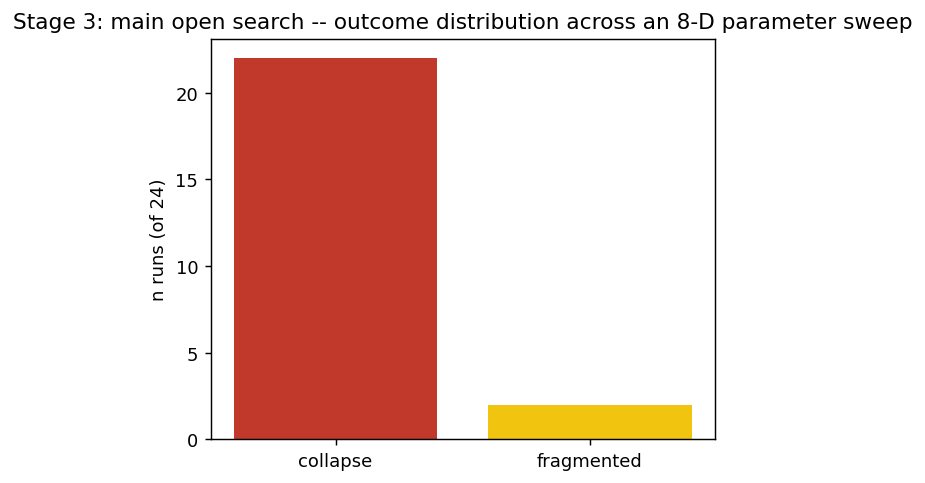
\includegraphics[width=0.75\textwidth]{figures/main/l12_fig1_stage3_outcome_distribution.png}
\caption{Level 1.2 Stage 3 main-search outcome distribution ($n=24$):
22 collapse, 2 fragmented, 0 viable. Descriptive: one run per (parameter
draw, seed) pair from an 8-dimensional Latin Hypercube sweep.}
\label{fig:l12-stage3-outcomes}
\end{figure}

\begin{figure}[htbp]
\centering
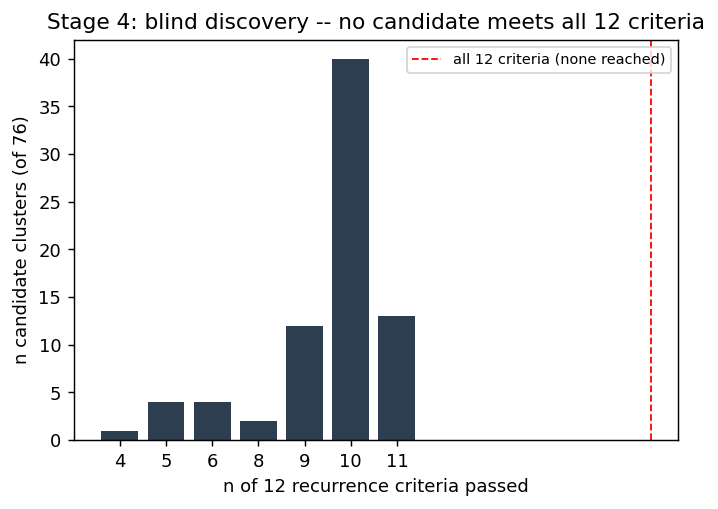
\includegraphics[width=0.75\textwidth]{figures/main/l12_fig2_recurrence_criteria.png}
\caption{Level 1.2 Stage 4: number of the twelve preregistered recurrence
criteria passed by each of 76 candidate clusters ($n=24$ pooled seed-runs).
No candidate passed all twelve; the best passed eleven.}
\label{fig:l12-recurrence-criteria}
\end{figure}

\begin{figure}[htbp]
\centering
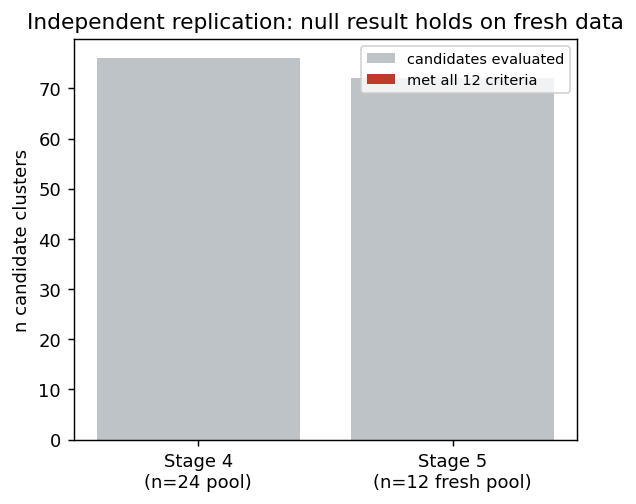
\includegraphics[width=0.85\textwidth]{figures/main/l12_fig3_discovery_vs_replication.png}
\caption{Level 1.2 Stage 4 discovery ($n=24$, 0/76 candidates) versus
Stage 5 independent fresh-seed confirmation ($n=12$, 0/72 candidates),
identical unmodified discovery pipeline. Descriptive null replication.}
\label{fig:l12-discovery-replication}
\end{figure}

\begin{figure}[htbp]
\centering
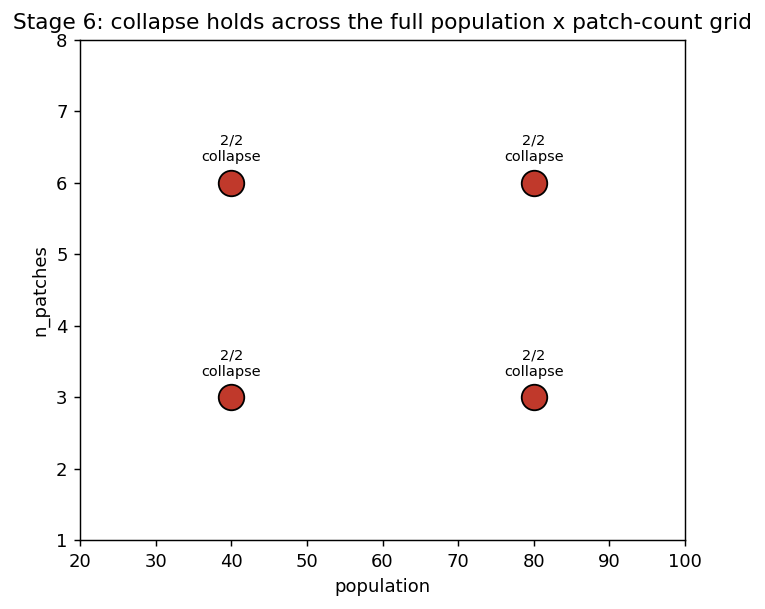
\includegraphics[width=0.8\textwidth]{figures/main/l12_fig4_scaling_grid.png}
\caption{Level 1.2 Stage 6 scaling-robustness grid: outcome label by
population $\times$ patch-count condition (8 runs, 2 seeds/condition).
Collapse in 8/8 runs.}
\label{fig:l12-scaling}
\end{figure}

\begin{figure}[htbp]
\centering
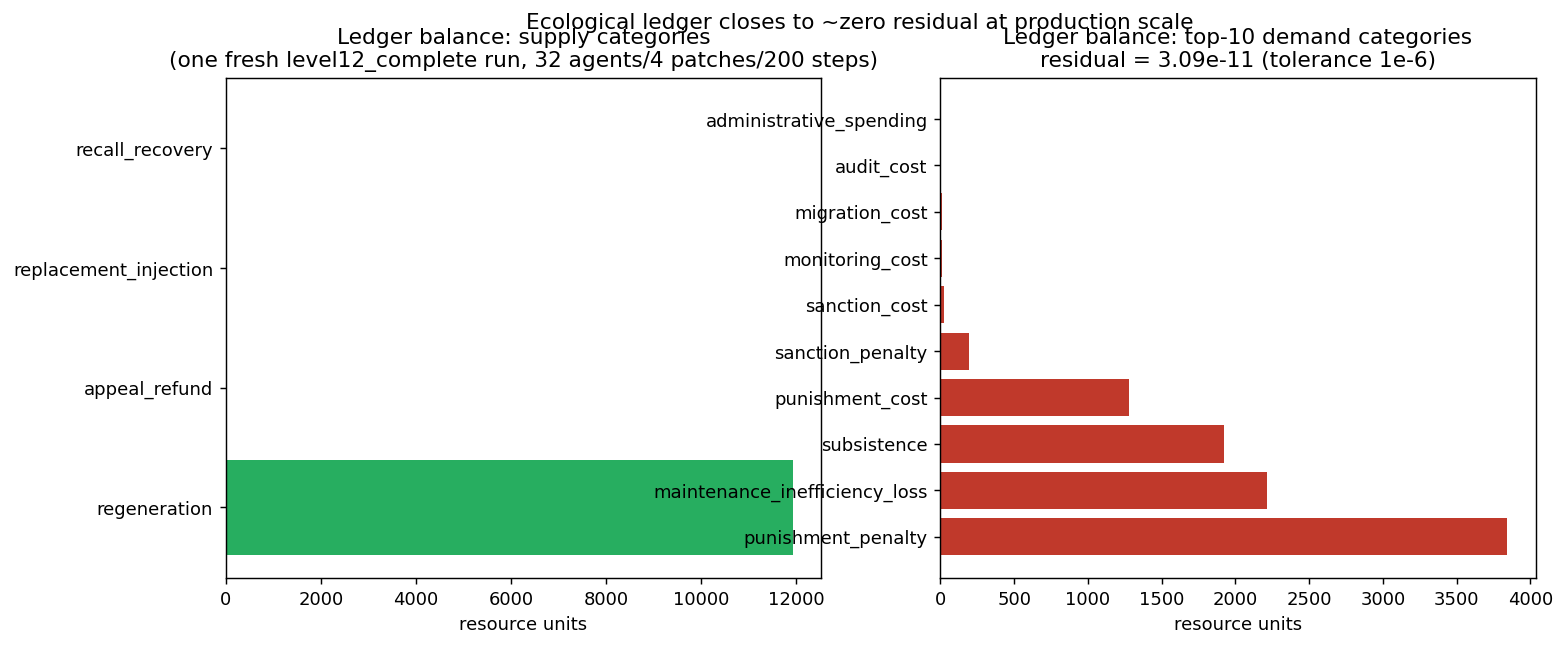
\includegraphics[width=0.95\textwidth]{figures/main/l12b_fig1_ledger_balance.png}
\caption{Level 1.2b ecological ledger: supply categories (left; dominated
by patch regeneration) and top-10 demand categories (right) for one fresh
diagnostic \texttt{level12\_complete} run. Residual $3.09\times10^{-11}$
against a documented tolerance of $10^{-6}$ on this run; across the full
576-run production design the maximum residual was $5.9\times10^{-9}$.}
\label{fig:l12b-ledger}
\end{figure}

\begin{figure}[htbp]
\centering
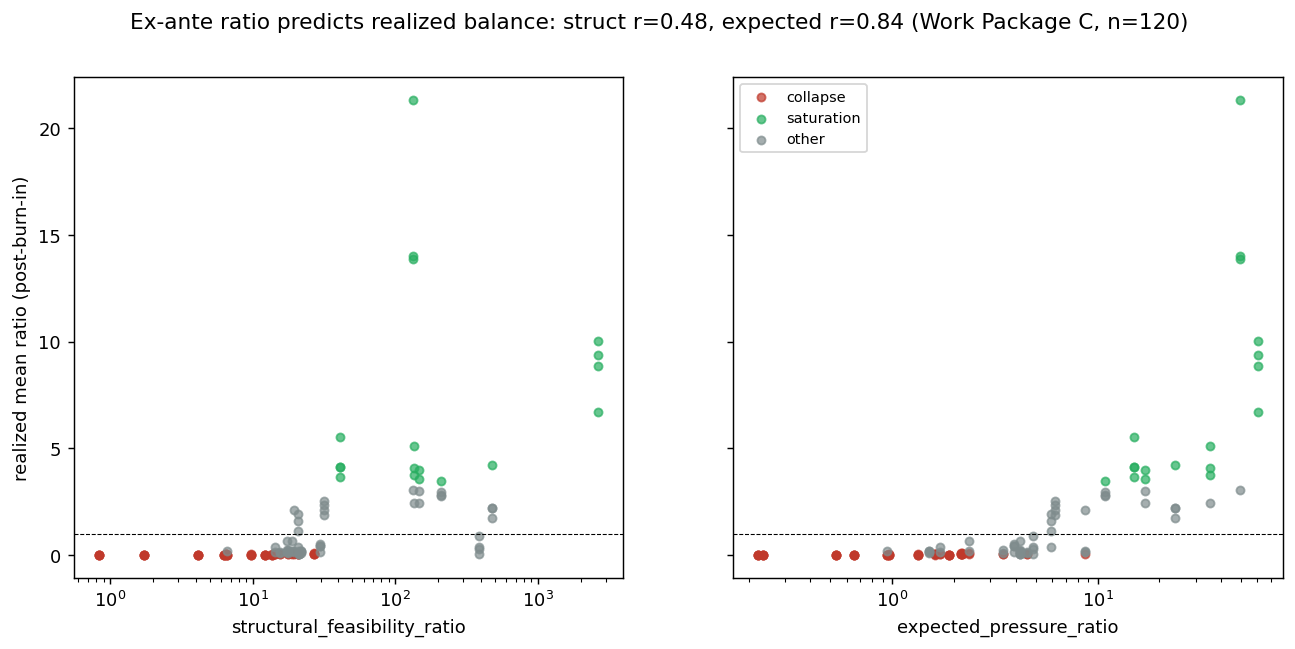
\includegraphics[width=0.75\textwidth]{figures/main/l12b_fig2_feasibility_ratios.png}
\caption{Ex-ante structural feasibility ratio and expected-pressure ratio
plotted against realized ecological balance ($n=120$ feasibility-map
runs). The expected-pressure ratio (Pearson $r\approx0.84$) tracks
realized balance substantially better than the structural ratio
($r\approx0.48$). Descriptive correlation, computed post hoc against
outcomes the ratios themselves never used for stratification.}
\label{fig:l12b-feasibility-ratios}
\end{figure}

\begin{figure}[htbp]
\centering
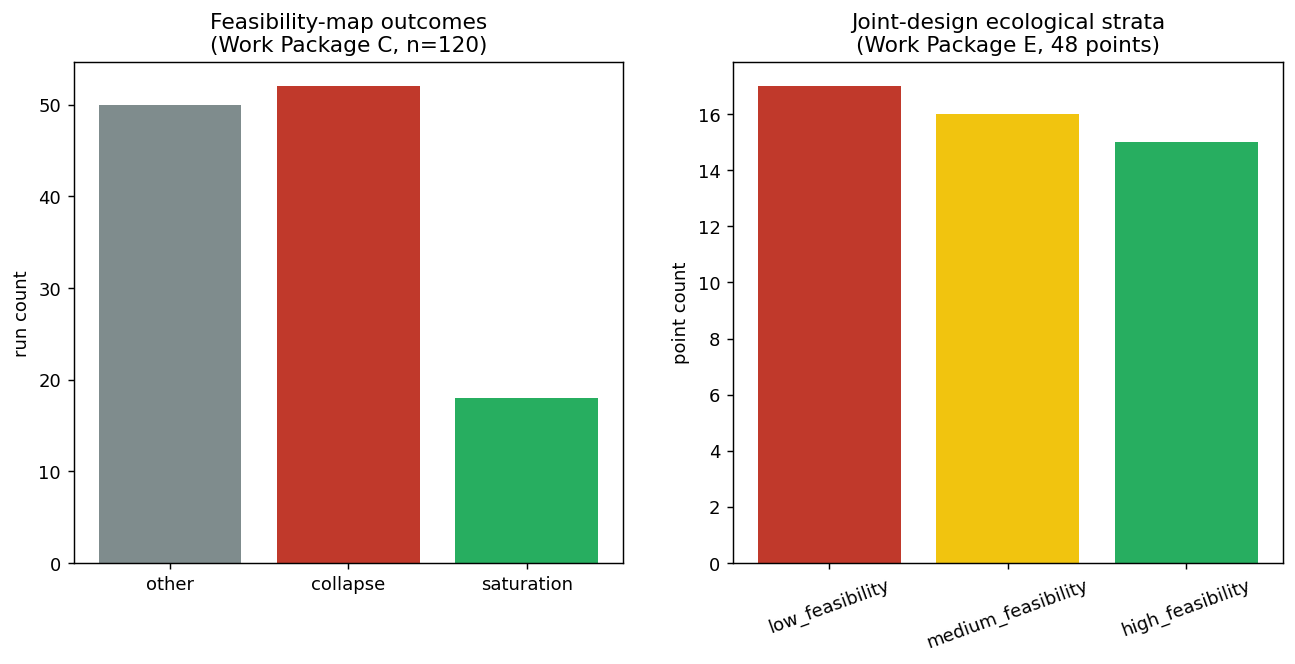
\includegraphics[width=0.85\textwidth]{figures/main/l12b_fig3_feasibility_strata.png}
\caption{Feasibility map and the tertile ecological strata (low/medium/
high expected-pressure ratio) frozen before the main joint discovery
design was generated.}
\label{fig:l12b-feasibility-strata}
\end{figure}

\begin{figure}[htbp]
\centering
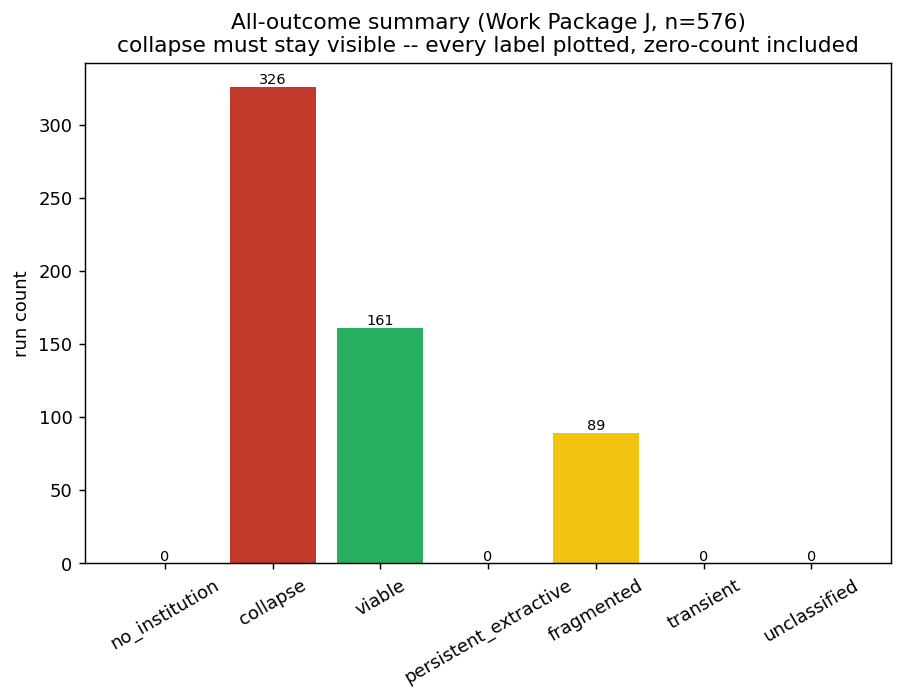
\includegraphics[width=0.75\textwidth]{figures/main/l12b_fig4_outcome_distribution.png}
\caption{Level 1.2b Work Package J complete all-outcome distribution
($n=576$), every label plotted including zero-count labels: collapse=326,
viable=161, fragmented=89, all others 0.}
\label{fig:l12b-outcome-distribution}
\end{figure}

\begin{figure}[htbp]
\centering
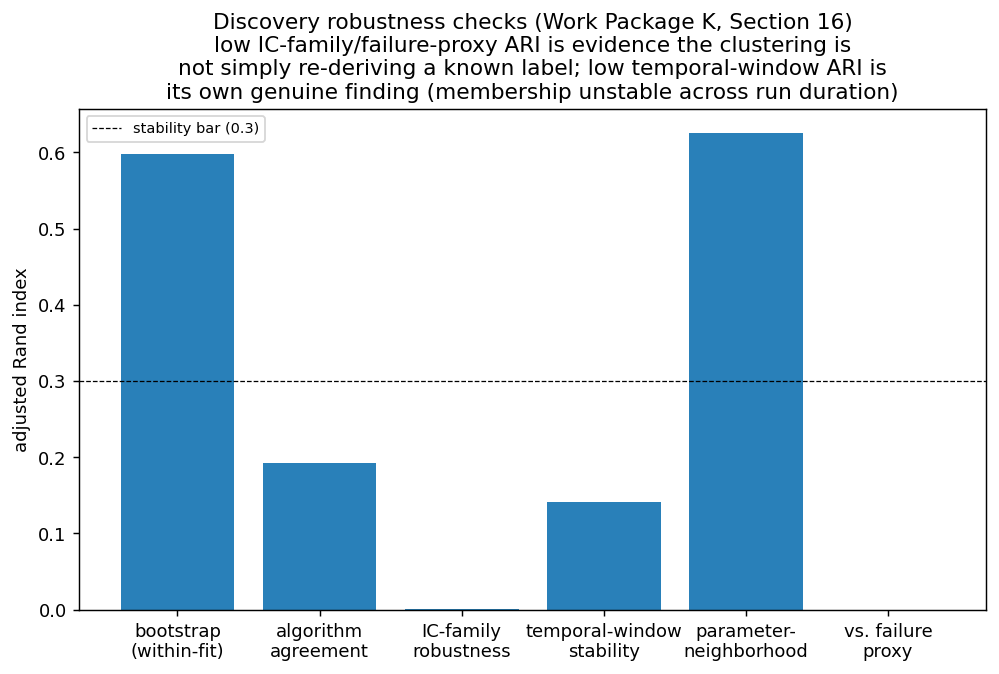
\includegraphics[width=0.85\textwidth]{figures/main/l12b_fig5_stability_metrics.png}
\caption{Level 1.2b discovery-pool clustering stability diagnostics:
bootstrap adjusted Rand index, pairwise algorithm-agreement adjusted Rand
index, missingness-strategy robustness, and temporal-window stability.
Descriptive fit diagnostics, not a causal claim.}
\label{fig:l12b-stability-metrics}
\end{figure}

\begin{figure}[htbp]
\centering
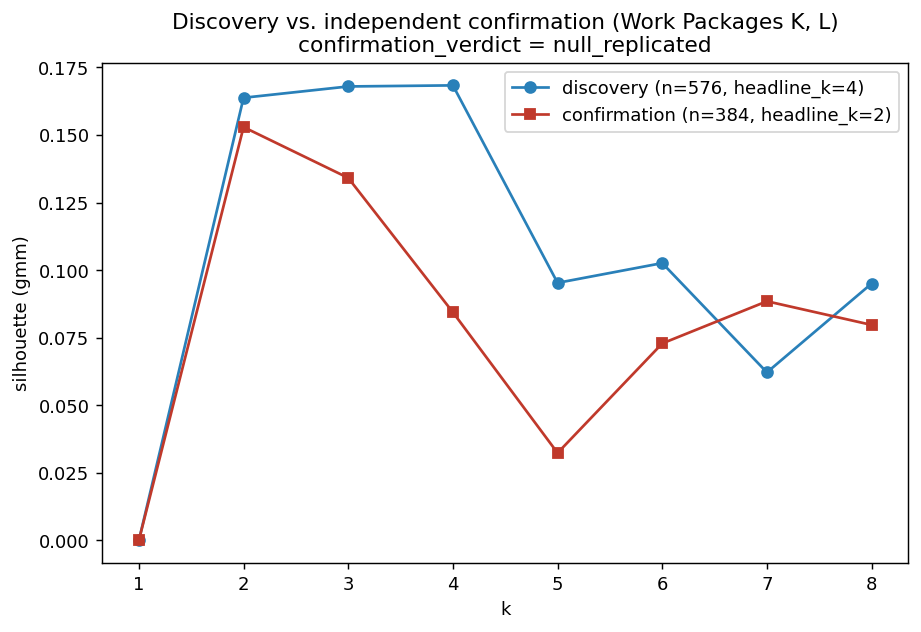
\includegraphics[width=0.75\textwidth]{figures/main/l12b_fig6_discovery_vs_confirmation.png}
\caption{Gaussian-mixture silhouette-by-$k$ curves: discovery pool
($n=576$, headline $k=4$) versus independent fresh confirmation pool
($n=384$, headline $k=2$), confirmation\_verdict=\texttt{null\_replicated}.
Descriptive null replication on disjoint data.}
\label{fig:l12b-discovery-confirmation}
\end{figure}

\begin{figure}[htbp]
\centering
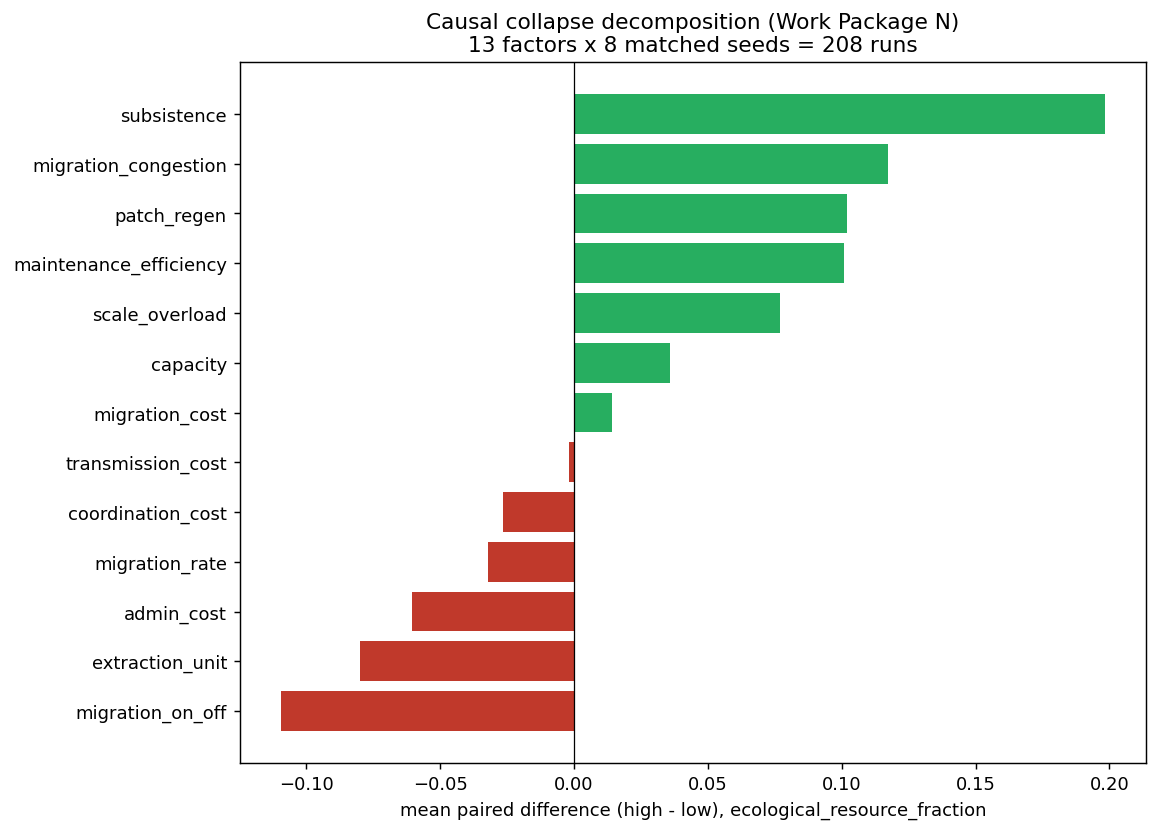
\includegraphics[width=0.9\textwidth]{figures/main/l12b_fig7_causal_ablation.png}
\caption{Work Package N thirteen-factor matched-seed causal-ablation
effect sizes on ecological-fraction outcomes ($n=208$ runs, 8 matched
pairs per factor). Causal evidence (matched-seed, \texttt{rng\_%
mode="mechanism\_substreams"}), distinct from every descriptive figure
above.}
\label{fig:l12b-causal-ablation}
\end{figure}

\subsection{Level 1.3 / Level 1.3b: the historically extended substrate}
\label{sec:results-l13}

\textbf{Historical effect on institutional response.} History causally and
persistently shapes institutional trajectories. Sham machinery validated
12/12 seeds byte-identical to control (Level 1.3b Stage 6); three of four
real history-erasure/reversal/equalization interventions produced real,
non-decaying, in several tests \textit{growing} final-sustained
divergence: \texttt{pressure\_memory\_only} 0.054, \texttt{entrenchment\_%
only} 0.072, \texttt{all\_history} 0.069 (mean $|S_{\text{obs}}|$ gap).
Level 1.3's own earlier, pooled-observational counterfactual (Stage 5:
erased-versus-base $\approx0.0027$, reversed-versus-base $\approx0.0116$)
pointed the same direction at smaller effect size, before purpose-designed
sham validation existed.

\textbf{Ordering effect: real but modest and direction-inconsistent.}
Level 1.3b Stage 3 (216 runs, purpose-designed factorial): 24.1\%
($S_{\text{obs}}$) and 32.4\% ($Z_{\text{obs}}$) of 108 matched pairwise
contrasts show a seed-clustered bootstrap CI excluding zero; direction is
consistent for one of three ordering-pair comparisons (27/36) and
inconsistent for the other two (20/36, 14/36). Level 1.3's own Stage 3 (72
runs, pooled design) found a comparable $\approx6$--$7.5\%$ relative
spread across six orderings.

\textbf{Discreteness, tested twice, rejected twice, more decisively the
second time.} Level 1.3's six-way verdict: \texttt{D\_continuum} (headline
$k{=}2$, silhouette 0.334, failed independent fresh-data reproduction:
log-likelihood $-1.29$ train versus $-6.05$ fresh). Level 1.3b's
eight-way verdict, from a purpose-designed pool and reusing Level 1.2b's
own frozen classifier unmodified: \texttt{D\_persistent\_continuum}
(headline $k{=}8$ by BIC, but silhouette never clears 0.15 across any
tested $k$, best $=0.143$ at $k{=}2$; cross-algorithm adjusted Rand index
0.016--0.357; cross-ecological-stratum adjusted Rand index $-0.043$ to
$-0.014$) (\cref{tab:l13-vs-l13b-discreteness}).

\textbf{$S_{\text{obs}}$--$Z_{\text{obs}}$ coupling: real, modest, and
weighting-sensitive.} Level 1.3 Stage 8 (pre-audit, $n=228$ pooled): Pearson
$r=0.888$, Spearman $\rho=0.913$. Level 1.3b Stage 9 (measurement-weighting
audit, $n=240$): equal-weight $r=0.264$, partial (controlling ecological
stratum) $r=0.272$, between-point $r=0.285$, within-point $r=0.261$,
leave-one-component-out range 0.175--0.307, PCA-weighted $r=0.136$ (a
genuine outlier, roughly half the equal-weight figure). Zero shared
component dimensions between the two composites, confirmed directly; PCA
does not cleanly recover an $S$/$Z$ axis split (PC1 loaded by both
legitimacy channels together).

\textbf{Bargaining activation, repaired and confirmed at scale.} 166/240
(69.2\%) Stage 4 runs activate under \texttt{repeated\_shocks} pressure;
20/24 (83\%) Stage 2 calibration cells land in the target range at
unmodified Level 1.1/1.2b defaults --- an observer-construction fix, not a
generative recalibration.

\begin{table}[htbp]
\centering
\caption{Discreteness testing, Level 1.3 versus Level 1.3b: both verdicts
reject discrete institutional families, reached via Level 1.2b's own
frozen classifier reused unmodified at both milestones.}
\label{tab:l13-vs-l13b-discreteness}
\adjustbox{max width=\textwidth}{\begin{tabular}{@{}llll@{}}
\toprule
\textbf{Metric} & \textbf{Level 1.3} & \textbf{Level 1.3b} & \textbf{Note} \\
\midrule
Design & pooled, post hoc (Stages 3--5) & purpose-designed (Stage 4) & 1.3b avoids 1.3's own confound \\
$n$ discovery pool & 216 & 240 & \\
Headline $k$ / selection rule & 2 (silhouette) & 8 (BIC) & different selection metrics led \\
Best silhouette (any $k$) & 0.334 ($k$=2) & 0.143 ($k$=2) & 1.3b never clears 0.15 floor \\
Bootstrap stability (mean ARI) & 0.917 & 0.752 & both clear 0.3 floor \\
Cross-algorithm agreement (ARI) & 0.291 (mean) & 0.016--0.357 (range, excl.\ non-independent pair) & both weak \\
Fresh-data reproduction & failed ($-1.29\to-6.05$ log-lik.) & mixed (+3.11 gap, but continuous candidate ties it) & \\
Cross-stratum reproduction & not tested & $-0.043$ to $-0.014$ (ARI) & 1.3b only; near-zero/negative \\
Formal verdict & \texttt{D\_continuum} & \texttt{D\_persistent\_continuum} & same top-level label, independent evidentiary path \\
\bottomrule
\end{tabular}
}
\end{table}

\begin{table}[htbp]
\centering
\caption{Level 1.3b Stage 6 sham-controlled history-erasure/reversal/
equalization intervention: mean $|S_{\text{obs}}|$ gap versus control by
window (12 matched seeds per arm).}
\label{tab:history-intervention}
\adjustbox{max width=\textwidth}{\begin{tabular}{@{}lrrrr@{}}
\toprule
\textbf{Arm} & \textbf{Early} & \textbf{Middle} & \textbf{Late} & \textbf{Final-sustained} \\
\midrule
\texttt{sham\_identical\_state\_copy} & \multicolumn{4}{c}{12/12 seeds byte-identical to control at every window} \\
\texttt{pressure\_memory\_only} & n/r & n/r & n/r & 0.054 \\
\texttt{entrenchment\_only} & 0.0 & 0.017 & 0.065 & 0.072 \\
\texttt{legitimacy\_history\_only} & n/r & 0.009 & n/r & $\approx4\times10^{-12}$ \\
\texttt{all\_history} & n/r & n/r & n/r & 0.069 \\
\bottomrule
\end{tabular}
}

\medskip
\noindent\footnotesize n/r = not individually reported at that window in
\texttt{docs/level1.3b\_scientific\_note.md}; the qualitative pattern
(middle-window gaps 0.009--0.017, growing to final-sustained 0.054--0.072
across the three non-legitimacy arms) is reported in aggregate even where
a specific arm's own middle/late value is not.
\normalsize
\end{table}
